\chapter{การออกแบบระบบ และรายละเอียดการพัฒนา}
\label{chapter:system-detail}
\section{ภาพรวมของระบบ}
การทำงานของระบบจัดการโฆษณาแบบจำกัดจำนวนการคลิกและการแสดงโฆษณา จะประกอบไปด้วยหลาย ๆ เซอร์วิสที่ทำงานร่วมกัน เพื่อให้สามารถทำงานได้ตามฟังก์ชันหลักที่จำเป็น ดังนี้

\begin{figure}[!h]
	\centering
	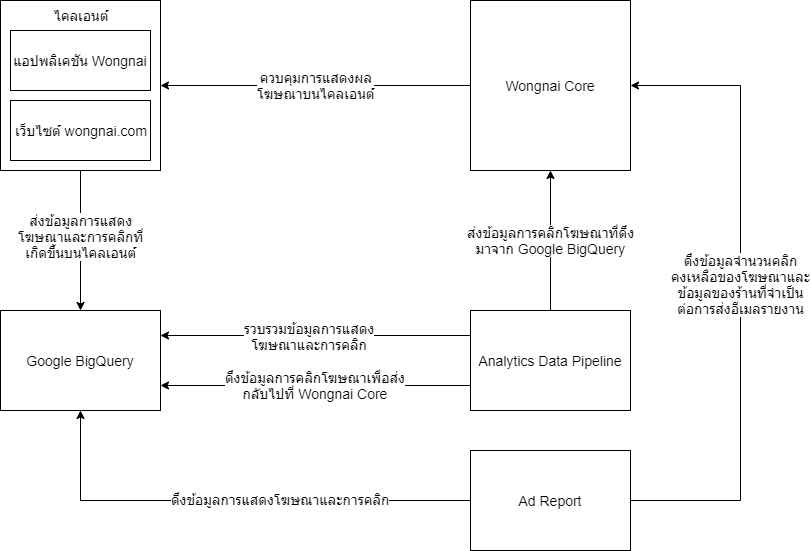
\includegraphics[width=1\textwidth]{ad-report-diagram.png}  
	\caption{แผนผังภาพรวมการทำงานของระบบจัดการโฆษณาแบบจำกัดจำนวนการคลิกและการแสดงโฆษณา}
	\label{Fig:adreport-diagram}
\end{figure}
	
โดย Wongnai Core เป็นเซอร์วิสขนาดใหญ่และเป็นเซอร์วิสหลักของ Wongnai ซึ่งเซอร์วิสนี้เคยเป็นเซอร์วิสที่มีสถาปัตยกรรมแบบ Monolith เมื่อนานมาแล้ว กล่าวคือระบบของ Wongnai ทุกอย่างเคยถูกพัฒนาใน Wongnai Core เพียงแค่ที่นี้ที่เดียว ไม่มีการแยกออกเป็นเซอร์วิสย่อย ๆ ภายหลังเมื่อระบบของ Wongnai มีขนาดใหญ่มากขึ้น แต่ละ Squad ไม่สามารถทำงานได้อย่างคล่องตัว จึงจำเป็นต้องแยกส่วนการทำงานออกมาเป็นอีกเซอร์วิสย่อยโดยใช้สถาปัตยกรรมไมโครเซอร์วิส อย่างไรก็ตามถ้าการแยกเซอร์วิสย่อยออกมา ไม่ทำให้ทีมทำงานได้คล่องตัวขึ้นเลย ก็ไม่จำเป็นจะต้องแยกเซอร์วิสก็ได้ สามารถพัฒนาฟังก์ชันใหม่ใน Wongnai Core ได้เลย ~\cite{wnservice}

ในการปฏิบัติงานนี้ ได้เล็งเห็นว่าหากเพิ่มฟังก์ชันที่สามารถส่งอีเมลรายงานผลการโฆษณากลับไปยังลูกค้าโดยอัตโนมัติได้ จะทำให้ Wongnai Core มีขนาดใหญ่เกินไป, การ Build เซอร์วิสนั้นนานมากขึ้น และเสียเวลาในการพัฒนาฟังก์ชันมากขึ้น จึงมีได้ตกลงกันว่าควรจะแยกออกเป็นอีกเซอร์วิสหนึ่ง ที่สามารถจัดการในเรื่องการส่งอีเมลรายงานผลการโฆษณากลับไปยังลูกค้าโดยอัตโนมัติโดยเฉพาะ แต่อย่างไรก็ตาม ระบบจัดการโฆษณาเดิมที่มีอยู่แล้ว อยู่ที่ Wongnai Core และมีความเห็นจาก Squad ว่า การนำฟังก์ชันส่วนนี้ออกมานั้นทำให้เสียเวลาในการพัฒนามากเกินไป จึงได้พัฒนาฟังก์ชันการจำกัดการแสดงโฆษณาของร้านด้วยจำนวนการคลิกโฆษณาไว้ที่ Wongnai Core เนื่องจากจำเป็นที่จะต้องมีทั้งการพัฒนาจากเซอร์วิสเดิม และการสร้างเซอร์วิสใหม่ จึงได้มีการแบ่งหน้าที่รับผิดชอบงานในส่วนต่าง ๆ ดังที่ปรากฏในตารางที่ 3.1

\begin{table}[!h]    
	\centering
	\begin{tabular}{|c|c|l|}
		\hline
		\textbf{เซอร์วิส} & \textbf{ผู้รับผิดชอบ} & \multicolumn{1}{c|}{\textbf{หมายเหตุ}} \\ \hline
		Wongnai Core & พนักงาน, นักศึกษา & \begin{tabular}[c]{@{}l@{}}นักศึกษารับผิดชอบในการพัฒนา API สำหรับให้\\ Ad Report ขอข้อมูลเพิ่มเติมในการสร้างรายงาน\end{tabular} \\ \hline
		Analytics Data Pipeline & พนักงาน, นักศึกษา & \begin{tabular}[c]{@{}l@{}}นักศึกษารับผิดชอบในการสร้างโปรเซสเซอร์แยก \\ข้อมูลเหตุการณ์ที่เกี่ยวกับโฆษณาบน Wongnai\end{tabular} \\ \hline
		Ad Report & พนักงาน, นักศึกษา & \begin{tabular}[c]{@{}l@{}}นักศึกษารับผิดชอบพัฒนาเซอร์วิสนี้เป็นส่วนใหญ่\\ โดยมี Software Engineer (Frontend) และ UX/UI\\ Designer เป็นผู้ช่วยเหลือในการสร้างรูปแบบของ \\อีเมลและรายงาน\end{tabular} \\ \hline
	\end{tabular}
	\caption{ตารางการแบ่งหน้าที่รับผิดชอบงานในส่วนต่าง ๆ ของระบบ}
	\label{Table:role}
\end{table}

\section{รายละเอียดการพัฒนาระบบ}
รายละเอียดของแต่ละเซอร์วิสที่เกี่ยวข้องกับระบบจัดการโฆษณาแบบจำกัดจำนวนการคลิกและการแสดงโฆษณา และรายละเอียดส่วนที่ได้พัฒนาเพิ่มขึ้นมา จะเป็นไปดังต่อไปนี้

\begin{enumerate}
	\item Wongnai Core
	
	Wongnai Core เป็นเซอร์วิสขนาดใหญ่และเป็นเซอร์วิสหลักของ Wongnai พัฒนาด้วยภาษา Java โดยหน้าที่ของ Wongnai Core ที่เกี่ยวข้องกับระบบจัดการโฆษณาแบบจำกัดจำนวนการคลิกและการแสดงโฆษณาโดยตรง ได้แก่
	
	\begin{itemize}
		\item จัดการโฆษณาที่แสดงบน Wongnai โดยสามารถจัดการได้จากหน้าแอดมินของ Wongnai Core ซึ่งเป็นหน้าแอดมินที่ใช้งานมานานแล้ว โดยจะเป็นหน้าแอดมินดังกล่าว จะถูกใช้โดยพนักงานที่เกี่ยวข้องกับการโฆษณาบน Wongnai สามารถเพิ่ม-ลบร้านที่จะลงโฆษณา, เลือกตำแหน่งที่จะแสดงโฆษณาบน Wongnai, สามารถแก้ไขข้อความโฆษณา และสามารถกำหนดช่วงเวลาที่จะแสดงโฆษณาได้
		\item ประมวลผลเมื่อได้รับข้อมูลจำนวนคลิกของโฆษณา เพื่อนำมาอัปเดตในฐานข้อมูลของ Wongnai Core จากนั้นจึงทำการพิจารณาว่าควรจะนำโฆษณาที่แสดงอยู่ออกหรือไม่ โดยดูจากจำนวนคลิกของโฆษณาว่าเกินกว่าที่จำกัดไว้ตามที่ตกลงกันหรือไม่ ถ้าเกินก็จะหยุดการแสดงโฆษณานั้น ๆ
		\item รอรับการร้องขอข้อมูลจากเซอร์วิส Ad Report เพื่อนำข้อมูลไปใช้ในการสร้างรายงานที่สมบูรณ์ส่งกลับไปยังเจ้าของโฆษณา ซึ่งประกอบไปด้วย ชื่อร้าน, อีเมลของร้าน, จำนวนคลิกโฆษณาของร้านที่ใช้ไปแล้ว และจำนวนคลิกโฆษณาของร้านซื้อไว้
	\end{itemize}

	สำหรับส่วนที่ได้รับผิดชอบโดยตรงคือ การสร้าง API ใน Wongnai Core เพื่อให้เซอร์วิส Ad Report สามารถขอข้อมูลเพิ่มเติมในการส่งอีเมลรายงานผลการโฆษณา ในที่นี้ได้ใช้โปรโตคอล HTTP เป็นตัวกลางในการสื่อสาร โดยรายละเอียดของ API ที่ได้พัฒนาเพิ่มขึ้นมา จะเป็นไปดังต่อไปนี้
	
	\begin{itemize}
		\item API สำหรับดึงข้อมูลของร้าน
		
		\begin{table}[!h]
			\centering
			\begin{tabular}{|c|c|c|c|}
				\hline
				\textbf{API Name} & \textbf{Method} & \multicolumn{2}{c|}{\textbf{URL}} \\ \hline
				businessInformation & GET & \multicolumn{2}{c|}{https://\{url\}/cb/\_/listing-ads/business/\{businessId\}} \\ \hline
				\multicolumn{4}{|c|}{\textbf{Request Path Parameter}} \\ \hline
				\textbf{Parameter Name} & \textbf{M/O} & \textbf{SV/MV} & \textbf{Data Type} \\ \hline
				businessId & M & SV & String \\ \hline
				\multicolumn{4}{|c|}{\textbf{Response Parameter}} \\ \hline
				\textbf{Parameter Name} & \textbf{M/O} & \textbf{SV/MV} & \textbf{Data Type} \\ \hline
				businessName & M & SV & String \\ \hline
				businessEmail & O & SV & String \\ \hline
				\multicolumn{4}{|r|}{*M: Mandatory; O: Optional; *SV: Single value; MV: Multi Value;} \\ \hline
			\end{tabular}
			\caption{ตารางรายละเอียดของ API สำหรับดึงข้อมูลของร้าน}
			\label{Table:api-detail-1}
		\end{table}
		
		\item API สำหรับดึงข้อมูลจำนวนคลิกโฆษณาของร้าน
		
		\begin{table}[!h]
			\centering
			\begin{tabular}{|c|c|c|c|}
				\hline
				\textbf{API Name} & \textbf{Method} & \multicolumn{2}{c|}{\textbf{URL}} \\ \hline
				clickPackInformation & GET & \multicolumn{2}{c|}{https://\{url\}/cb/\_/listing-ads/current-used-click-pack/\{businessId\}} \\ \hline
				\multicolumn{4}{|c|}{\textbf{Request Path Parameter}} \\ \hline
				\textbf{Parameter Name} & \textbf{M/O} & \textbf{SV/MV} & \textbf{Data Type} \\ \hline
				businessId & M & SV & String \\ \hline
				\multicolumn{4}{|c|}{\textbf{Response Parameter}} \\ \hline
				\textbf{Parameter Name} & \textbf{M/O} & \textbf{SV/MV} & \textbf{Data Type} \\ \hline
				clickUsed & O & SV & String \\ \hline
				clickPuchased & O & SV & String \\ \hline
				\multicolumn{4}{|r|}{*M: Mandatory; O: Optional; *SV: Single value; MV: Multi Value;} \\ \hline
			\end{tabular}
			\caption{ตารางรายละเอียดของ API สำหรับดึงข้อมูลจำนวนคลิกโฆษณาของร้าน}
			\label{Table:api-detail-2}
		\end{table}
	\end{itemize}
		

	\item Analytics Data Pipeline
	
	Analytics Data Pipeline เป็นเซอร์วิสขนาดเล็กที่พัฒนาด้วยภาษา Python ปกติไคลเอนต์จะส่งข้อมูลเหตุการณ์ต่าง ๆ ที่เกิดขึ้นใน Wongnai มาเก็บใน Google BigQuery ซึ่งข้อมูลเหตุการณ์ต่าง ๆ นั้นมีหลายประเภทและมีปริมาณที่เยอะมากใน 1 วัน สาเหตุที่ใช้ Google BigQuery นั้นสืบเนื่องมาจากต้องการที่จะลดปัญหาจากปริมาณข้อมูลที่เยอะ ทำให้การดูแลรักษาฐานข้อมูล ทั้งในเรื่องของประสิทธิภาพและอื่น ๆ ทำได้ยากและมีค่าใช้จ่ายที่สูง โดย Google BigQuery เป็นเทคโนโลยีคลังข้อมูลที่ให้บริการอยู่บน Cloud ทำให้สามารถตัดปัญหาเรื่องการดูแลรักษาได้ทันที อย่างไรก็ตามข้อมูลเหตุการณ์ต่าง ๆ ที่ถูกส่งเข้ามาใน Google BigQuery จะถูกเก็บไว้ในตารางเดียวกันทั้งหมด ทำให้ตารางนั้นเป็นตารางที่มีข้อมูลมหาศาล และการดึงข้อมูลจาก Google BigQuery หนึ่งครั้ง จะต้องเสียค่าใช้จ่ายตามขนาดของข้อมูลในตาราง การดึงข้อมูลออกมาจากตารางใหญ่ โดยที่ใช้ข้อมูลเพียงแค่บางส่วนจะทำให้สูญเสียเครดิตไปโดยไม่จำเป็น Analytics Data Pipeline จึงถูกพัฒนาขึ้นเพื่อแก้ไขปัญหาในจุดนี้ ภายในเซอร์วิสนี้จะประกอบไปด้วยโปรเซสเซอร์ต่าง ๆ ซึ่งเป็นคลาสที่เอาไว้แยกข้อมูลแต่ละประเภทออกจากตารางใหญ่ สำหรับส่วนที่ได้รับผิดชอบโดยตรงคือ การเพิ่มโปรเซสเซอร์ที่สามารถแยกข้อมูลเหตุการณ์ที่เกี่ยวกับโฆษณาบน Wongnai โดยเราต้องทำการเพิ่มตารางใหม่ที่ต้องการใน Google BigQuery ก่อน จากนั้นจึงสร้างโปรเซสเซอร์ที่เอาไว้แยกข้อมูลขึ้นมา โดยจะต้องสร้าง Query String ที่เป็น SQL จากนั้นโปรเซสเซอร์ส่ง Query String ไปยัง Google BigQuery อีกที ซึ่ง Query String ที่จะใช้ จะเป็นการเลือกข้อมูลส่วนที่ต้องการออกมาก่อน เช่น "SELECT ... FROM ... WHERE ... GROUP BY ..." จากนั้นจึงนำข้อมูลส่วนที่แยกออกมาใส่ไปในตารางใหม่โดยใช้คำสั่ง "INSERT INTO ..."
	
	\begin{figure}[!h]
		\centering
		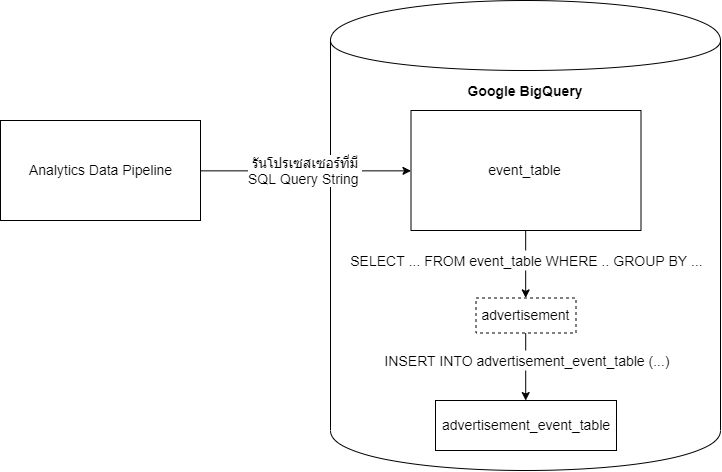
\includegraphics[width=0.95\textwidth]{analytics-data-pipeline}  
		\caption{แผนผังภาพรวมการทำงานของเซอร์วิส Analytics Data Pipeline}
		\label{Fig:analytics-data-pipeline}
	\end{figure}
	
	โปรเซสเซอร์ที่เพิ่มขึ้นมาจะทำให้ได้ตารางข้อมูลที่มีขนาดเล็กลง และมีเฉพาะส่วนที่เราต้องการนำไปใช้จริง ๆ ในที่นี้ได้เพิ่มโปรเซสเซอร์แยกเฉพาะข้อมูลเหตุการณ์ที่เกี่ยวกับโฆษณาบน Wongnai ออกมาเก็บไว้ในอีกตารางหนึ่งใน Google BigQuery เพื่อให้สะดวกต่อการนำไปใช้ต่อและลดค่าใช้จ่ายเนื่องจากไม่จำเป็นต้องไปดึงข้อมูลจากตารางใหญ่ โดยโปรเซสเซอร์นี้จะถูกรันทุก ๆ หนึ่งวันเพื่อเป็นการอัปเดตข้อมูลในตารางเล็กให้ทันปัจจุบัน
	
	\begin{table}[!h]
		\centering
		\begin{tabular}{|c|c|c|}
			\hline
			\textbf{Field name} & \textbf{Data Type} & \textbf{Description} \\ \hline
			Timestamp & TIMESTAMP & วันเวลาที่เกิดเหตุการณ์ \\ \hline
			EventLabel & STRING & ID ของร้าน \\ \hline
			EventAction & STRING & \begin{tabular}[c]{@{}c@{}}ประเภทของเหตุการณ์ที่เกิดขึ้น\\ ได้แก่ Click กับ Impression\end{tabular} \\ \hline
			App & STRING & \begin{tabular}[c]{@{}c@{}}Platform ที่เกิดเหตุการณ์ ได้แก่\\ Web, iOS และ Android\end{tabular} \\ \hline
			SearchResultView & STRING & \multirow{4}{*}{ตำแหน่งที่เกิดเหตุการณ์} \\ \cline{1-2}
			BusinessLandingDomain & STRING &  \\ \cline{1-2}
			Section & STRING &  \\ \cline{1-2}
			ScreenName & STRING &  \\ \hline
			Count & INTEGER & จำนวนครั้งที่เกิดเหตุการณ์ \\ \hline
		\end{tabular}
		\caption{Schema ของตารางที่แยกออกมาเพื่อเก็บข้อมูลเหตุการณ์ที่เกี่ยวกับโฆษณาบน Wongnai}
		\label{Table:schema-ad}
	\end{table}
		
	วิธีการตั้งค่าให้โปรเซสเซอร์ทำงานทุกวันโดยอัตโนมัติ จะใช้วิธีการทำ Task โดยอัตโนมัติด้วย CronJob ที่ Kubernetes ได้ โดยการเขียนไฟล์ .yaml ที่เอาไว้ตั้งค่าให้กับ Kubernetes 
	
	\begin{figure}[!h]
	 	\centering
	 	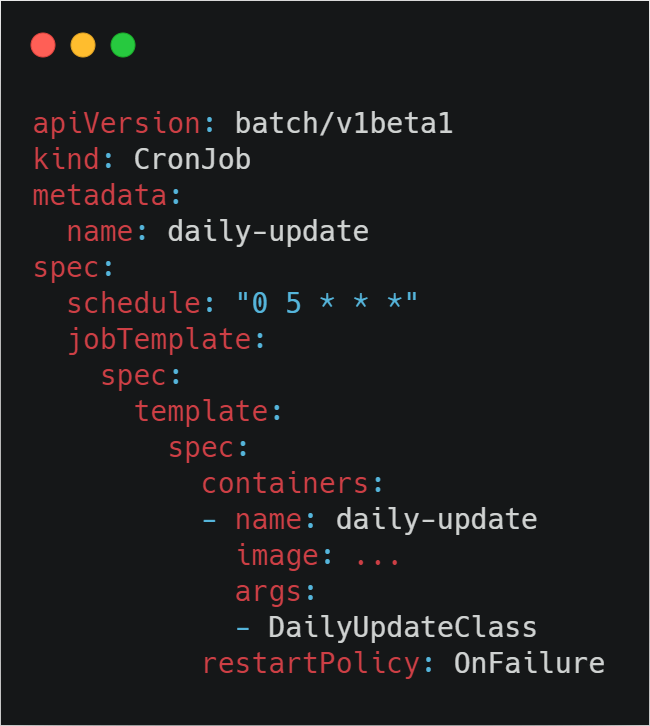
\includegraphics[width=0.475\textwidth]{cronjob1}  
	 	\caption{ตัวอย่างการตั้งค่า Kubernetes ให้รัน Task โดยอัตโนมัติด้วย CronJob}
	 	\label{Fig:cronjob1}
	\end{figure}
 
 	เราสามารถให้ตั้งค่า Kubernetes ให้รัน Task โดยอัตโนมัติได้ด้วย CronJob โดยตั้งเวลาที่ต้องการได้ที่ฟิลด์ schedule จากตัวอย่างรูปที่ 3.3 ได้ตั้งไว้ให้รันทุก ๆ วันตอน 13.00 น. เวลาประเทศไทย จุดสังเกตที่สำคัญคือ การตั้งเวลาต้องสังเกตด้วยว่าเครื่องที่เป็นเซิร์ฟเวอร์ที่จะรัน Task ใช้เขตเวลาอะไร ในที่นี้เขตเวลาของเครื่องจะเป็น UTC+0 จึงต้องคำนวณเวลาก่อนที่จะตั้งค่าลงไปในฟิลด์ schedule นอกจากนี้ หน้าที่อีกอย่างหนึ่งที่สำคัญของเซอร์วิสนี้ คือการนำข้อมูลเหตุการณ์ที่เกี่ยวกับโฆษณาบน Wongnai ที่แยกออกไปเก็บในตารางขนาดเล็กแล้ว ส่งไปอัปเดตที่ฐานข้อมูลของ Wongnai Core ทุก ๆ วัน เพื่อให้ Wongnai Core นำข้อมูลส่วนนี้ไปประมวลผลต่อตามที่กล่าวไว้ด้านบน
	
	\item Ad Report
	
	Ad Report เป็นเซอร์วิสใหม่ที่ถูกพัฒนาด้วยภาษา Java ร่วมกับ Spring Boot ทำหน้าที่สร้างอีเมลรายงานผลการโฆษณาที่ประกอบไปด้วยข้อมูลต่าง ๆ โดยภายในเซอร์วิสนี้ จะประกอบไปด้วยฟังก์ชันการทำงานหลัก 4 อย่าง ได้แก่
	\begin{itemize}
		\item Statistics Updater
		
		ฟังก์ชัน Statistics Updater ทำหน้าที่ดึงข้อมูลเหตุการณ์ที่เกี่ยวกับโฆษณาบน Wongnai ที่เก็บไว้อยู่ใน Google BigQuery มาอัปเดตลงในฐานข้อมูลของ Ad Report โดยฟังก์ชันนี้จะทำการส่ง Query String ที่เป็น SQL ไปยังตารางขนาดเล็กที่เก็บข้อมูลเหตุการณ์ที่เกี่ยวกับโฆษณาใน Google BigQuery เพื่อนำข้อมูลในช่วงเวลาที่ต้องการออกม าจากนั้นนำข้อมูลที่ได้มาบันทึกลงในฐานข้อมูล โดย Schema ของตารางที่จะบันทึกข้อมูลเหตุการณ์ที่เกี่ยวกับโฆษณาในเซอร์วิส Ad Report จะเป็นไปดังต่อไปนี้
		
		\begin{table}[!h]
			\centering
			\begin{tabular}{|c|c|c|}
				\hline
				\textbf{Field name} & \textbf{Data Type} & \textbf{Description} \\ \hline
				id & BIGINT & ID ของเหตุการณ์ \\ \hline
				timestamp & DATETIME & วันเวลาที่เกิดเหตุการณ์ \\ \hline
				business\_id & BIGINT & ID ของร้านที่เกิดเหตุการณ์ \\ \hline
				number\_of\_impressions & BIGINT & จำนวนครั้งที่แสดงโฆษณาของร้าน \\ \hline
				number\_of\_clicks & BIGINT & จำนวนครั้งที่เกิดการคลิกไปที่โฆษณาของร้าน \\ \hline
			\end{tabular}
			\caption{Schema ของตารางที่เก็บข้อมูลเหตุการณ์ที่เกี่ยวกับโฆษณาบน Wongnai ในเซอร์วิส Ad Report}
			\label{Table:schema-ad-report-1}
		\end{table}
		
		กรณีที่ข้อมูลที่เข้ามาใหม่จากการอัปเดตเป็นข้อมูลของร้านที่ไม่เคยปรากฏอยู่ในฐานข้อมูลของ Ad Report (เป็นร้านที่ลงโฆษณากับ Wongnai เป็นครั้งแรก) ฟังก์ชันนี้ก็จะทำการเรียกใช้งานฟังก์ชัน Retrieve Data เพื่อร้องขอข้อมูลชื่อร้านและอีเมลของร้านที่เข้ามาใหม่จาก Wongnai Core จากนั้นจึงบันทึกข้อมูลของร้านที่ได้มาทั้งหมดลงในอีกตาราง ซึ่งตารางนี้จะทำหน้าที่ในการเก็บข้อมูลของร้านเพื่อนำไปประกอบในการสร้างรายงานและการส่งอีเมล 
		
		\begin{table}[!h]
			\centering
			\begin{tabular}{|c|c|c|}
				\hline
				\textbf{Field name} & \textbf{Data Type} & \textbf{Description} \\ \hline
				business\_id & BIGINT & ID ของร้าน \\ \hline
				business\_name & VARCHAR(255) & ชื่อร้าน \\ \hline
				business\_email & VARCHAR(255) & อีเมลของร้าน \\ \hline
			\end{tabular}
			\caption{Schema ของตารางที่เก็บข้อมูลร้านในเซอร์วิส Ad Report}
			\label{Table:schema-ad-report-2}
		\end{table}
		
		\item Report
		
		ฟังก์ชัน Report ทำหน้าที่สร้างรายงานที่จะส่งไปพร้อมกับอีเมลให้กับลูกค้า โดยฟังก์ชันนี้จะทำการสร้างรายงานเป็นไฟล์นามสกุล .pdf จากเทมเพลตของรายงานที่เตรียมไว้ โดยเทมเพลตของรายงานจะเป็นไฟล์ที่ถูกแก้ไขมาแล้วบางส่วนให้ตรงกับที่ UX/UI Designer ออกแบบไว้ ซึ่งการจัดการไฟล์ .pdf จะใช้ไลบรารี iText ~\cite{itext} มาช่วยในการทำงาน ส่วนการสร้างแผนภูมิจะใช้ไลบรารี XChart  ~\cite{xchart} สำหรับการทำงานของฟังก์ชัน Report นั้น จะเป็นไปตามรูปที่ 3.4
		
		\begin{figure}[!h]
			\centering
			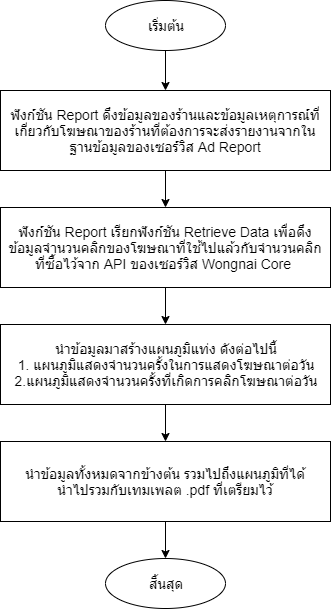
\includegraphics[width=0.5\textwidth]{report-diagram}  
			\caption{แผนผังการทำงานของฟังก์ชัน Report}
			\label{Fig:report-diagram}
		\end{figure}
		
		\item Report Email
		
		ฟังกชัน Report Email ทำหน้าที่สร้างอีเมลพร้อมกับแนบไฟล์รายงานที่ได้จากฟังก์ชัน Report ส่งไปยังอีเมลของลูกค้า ในที่นี้ได้ใช้คลาส EmailService ซึ่งเป็นคลาสที่มีอยู่แล้วในเฟรมเวิร์คของทาง Wongnai เพื่อทำการส่งอีเมล และใช้ Rocker Templates by Fizzed เป็นเทมเพลตสำหรับการเขียนอีเมลด้วย HTML ที่สามารถใช้คู่กับภาษา Java ได้ และมีประสิทธิภาพที่สูงในแง่ของความเร็วในการเรนเดอร์เทมเพลต ~\cite{rocker}
			
		\begin{figure}[!h]
			\centering
			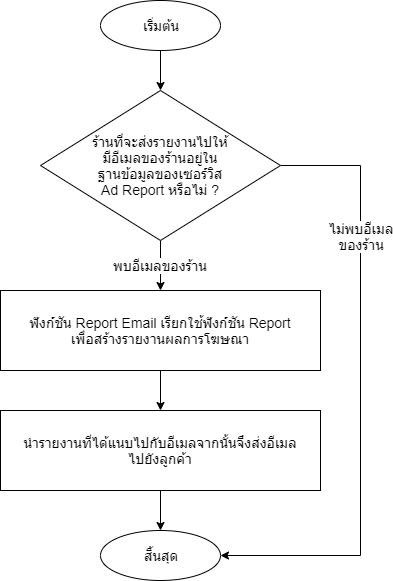
\includegraphics[width=0.65\textwidth]{email-diagram}  
			\caption{แผนผังการทำงานของฟังก์ชัน Report Email}
			\label{Fig:email-diagram}
		\end{figure}
			
		\item Retrieve Data
		
		ฟังกชัน Retrieve Data ทำหน้าหน้าที่ร้องขอข้อมูลที่จำเป็นจาก Wongnai Core เพื่อนำไปใช้ในการสร้างรายงานและการส่งอีเมลที่สมบูรณ์ โดยภายในฟังก์ชันนี้จะใช้คลาส RestTemplate ที่เป็นคลาสที่มีให้ในเฟรมเวิร์ค Spring Boot สำหรับการสร้างคำร้องขอแบบ REST ไปยัง API ของ Wongnai Core ทั้ง 2 API ได้แก่ API สำหรับดึงข้อมูลของร้าน กับ API สำหรับดึงข้อมูลจำนวนคลิกโฆษณาของร้าน ซึ่งได้อธิบายไว้แล้วก่อนหน้า
	\end{itemize}

	ภายในเซอร์วิส Ad Report จะมีคลาสที่เป็น ApplicationRunner อยู่อีกสองคลาส นอกเหนือจาก ApplicationRunner หลักที่เอาไว้รันเซอร์วิส Ad Report ถูกสร้างขึ้นมาเพื่อใช้ในการรัน Task โดยอัตโนมัติด้วย CronJob ที่ Kubernetes โดยทั้งสองคลาสจะมีรายละเอียดดังต่อไปนี้

	\begin{itemize}
		\item Weekly Report Email
		
		Weekly Report Email  เป็น ApplicationRunner Class ที่จะเรียกใช้งานฟังก์ชัน Report Email เพื่อสร้างรายงานผลการโฆษณาและส่งอีเมลกลับไปยังลูกค้าทุก ๆ สัปดาห์ ซึ่งจะส่งให้เฉพาะร้านที่ยังจำนวนคลิกโฆษณาคงเหลืออยู่ (กรณีที่ไม่มีจำนวนคลิกโฆษณาคงเหลือจะไม่ส่งแบบอัตโนมัติให้ เพราะถือว่าเป็นร้านที่โฆษณาหมดอายุไปแล้ว) โดยดูจากข้อมูลที่ร้องขอมาจากฟังก์ชัน Retrieve Data
	
		\begin{figure}[!h]
			\centering
			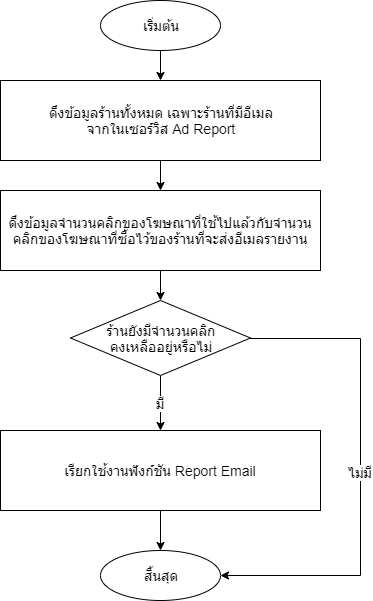
\includegraphics[width=0.55\textwidth]{weekly-report-email}  
			\caption{แผนผังการทำงานของ ApplicationRunner Class Weekly Report Email}
			\label{Fig:weekly-report-diagram}
		\end{figure}
	
		\item Daily Statistics Updater
	
		Daily Statistics Updater เป็น ApplicationRunner Class ที่จะเรียกใช้งานฟังก์ชัน Statistics Updater ทุก ๆ วัน เพื่ออัปเดตฐานข้อมูลเหตุการณ์ของโฆษณาบน Wongnai ของ Ad Report
	\end{itemize}

	นอกจากนี้เซอร์วิส Ad Report จะมีหน้าแอดมินสำหรับให้พนักงานที่เกี่ยวข้องมาใช้งานได้ โดยวิธีการพัฒนาหน้าแอดมินนั้นจะใช้เฟรมเวิร์ค admin-ui ที่ Wongnai มีให้อยู่แล้ว ซึ่ง admin-ui เป็นเฟรมเวิร์คที่ใช้ React ซึ่งเป็นไลบรารีสำหรับการสร้าง User Interface ให้กับเว็บไซต์ด้วยภาษา Javascript ~\cite{react} ถูกพัฒนามาสำหรับสร้างหน้าแอดมินให้กับเซอร์วิสใหม่ที่แยกออกมาจาก Wongnai Core โดยเราสามารถนำเฟรมเวิร์คนี้มาใช้ได้ทันที โดยที่ไม่จำเป็นต้องเขียนโค้ดอะไรเพิ่มเติมมากนัก แต่ในเซอร์วิส Ad Report นั้นต้องมี Action ในหน้าแอดมินที่สามารถส่งอีเมลรายงานด้วยตนเอง กรณีที่ระบบอัตโนมัติเกิดข้อผิดพลาดใด ๆ ก็ตาม ในการสร้าง Action ใน admin-ui จำเป็นต้องสร้าง API เพิ่มขึ้นมาในเซอร์วิส Ad Report โดย API ที่เพิ่มขึ้นมาจะทำการส่งอีเมลรายงานผลการโฆษณาให้กับลูกค้า ทันทีที่ได้รับการร้องขอ
	
	\begin{table}[!h]
		\centering
		\begin{tabular}{|c|c|c|c|}
			\hline
			\textbf{API Name} & \textbf{Method} & \multicolumn{2}{c|}{\textbf{URL}} \\ \hline
			sendWeeklyReportEmail & POST & \multicolumn{2}{l|}{\begin{tabular}[c]{@{}l@{}}https://\{url\}/admin/\\ business-information/\\ send-weekly-report-email/\\ \{buinessId\}\end{tabular}} \\ \hline
			\multicolumn{4}{|c|}{\textbf{Request Path Parameter}} \\ \hline
			\textbf{Parameter Name} & \textbf{M/O} & \textbf{SV/MV} & \textbf{Data Type} \\ \hline
			businessId & M & SV & String \\ \hline
		\end{tabular}
	\caption{ตารางรายละเอียดของ API สำหรับการสร้าง Action ส่งอีเมลรายงานผลการโฆษณาในหน้าแอดมิน}
	\label{Table:api-detail-3}
	\end{table}

	เฟรมเวิร์ค admin-ui จะคอยจัดการสิทธิ์การเข้าถึงหน้าแอดมินให้ โดยที่เราไม่จำเป็นต้องแนบพารามิเตอร์ใดเพิ่มเติม ๆ เข้าไปในคำร้องขอเพื่อยืนยันสิทธิ์การเข้าถึงหน้าแอดมิน เมื่อเราทำการส่งคำร้องขอไปที่ API นี้แล้ว ถ้าส่งอีเมลสำเร็จ จะได้คำตอบกลับ HTTP ที่มีสถานะเป็น 200 OK กลับมา แต่ถ้าไม่สำเร็จจะได้คำตอบกลับที่มีสถานะเป็น 4XX หรือ 5XX กลับมา ขึ้นอยู่กับว่าภายในเกิดข้อผิดพลาดอะไร
\end{enumerate}

เซอร์วิสทั้งหมดที่กล่าวมาทั้งหมดจะถูกทำให้เป็นคอนเทนเนอร์โดยใช้ Docker เพื่อให้สะดวกต่อการ Deploy ด้วย Kubernetes โดยแต่ละเซอร์วิสก็จะมี Dockerfile ไว้สำหรับการสร้างคอนเทนเนอร์อิมเมจของเซอร์วิสนั้น ๆ สำหรับ Ad Report ซึ่งเป็นเซอร์วิสใหม่นั้น ได้ทำการเพิ่มไฟล์ .gitlab-ci.yml สำหรับใช้งาน Gitlab CI/CD เพื่อให้ทำการ Build โค้ด, สร้างคอนเทนเนอร์อิมเมจ, นำอิมเมจไปจัดเก็บใน Private Image Registry ซึ่งเป็นพื้นที่สำหรับจัดเก็บอิมเมจของ Wongai และ Deploy เซอร์วิสโดยอัตโนมัติ สำหรับการตั้งค่าให้กับ Kubernetes เพื่อนำคอนเทนเนอร์อิมเมจที่สร้างมาไป Deploy เป็นบนเซิร์ฟเวอร์ จะมี Project Eastern ซึ่งเป็นไลบรารีที่เป็นเทมเพลตในการตั้งค่า Kubernetes และช่วยจัดการ Environment ที่จะ Deploy ให้ ~\cite{eastern} 

\begin{figure}[!h]
	\centering
	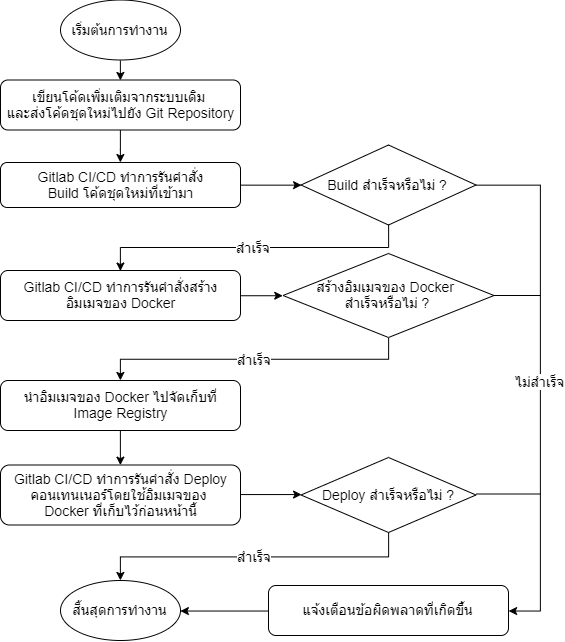
\includegraphics[width=1\textwidth]{gitlab-flow.png}  
	\caption{แผนผังวิธีการ Deploy โค้ดชุดใหม่ของเซอร์วิส Ad Report}
	\label{Fig:adreport-diagram}
\end{figure}